\documentclass[final]{beamer}
%% Possible paper sizes: a0, a0b, a1, a2, a3, a4.
%% Possible orientations: portrait, landscape
%% Font sizes can be changed using the scale option.
\usepackage[size=a0,orientation=portrait]{beamerposter}

\usetheme{gemini}
\usecolortheme{seagull}
\useinnertheme{rectangles}

% ====================
% Packages
% ====================

\usepackage[utf8]{inputenc}
\usepackage{graphicx}
\usepackage{booktabs}
\usepackage{tikz}
\usepackage{pgfplots}
\usepackage{wrapfig,lipsum}
\usepackage{cleveref}
% \usepackage{sidecap}

% ====================
% Lengths
% ====================

% If you have N columns, choose \sepwidth and \colwidth such that
% (N+1)*\sepwidth + N*\colwidth = \paperwidth
\newlength{\sepwidth}
\newlength{\colwidth}
\setlength{\sepwidth}{0.03\paperwidth}
\setlength{\colwidth}{0.45\paperwidth}
% \setlength\abovecaptionskip{-5pt}
\setlength\belowcaptionskip{-5pt}
\setlength{\headsep}{-5pt}

\newcommand{\separatorcolumn}{\begin{column}{\sepwidth}\end{column}}

% ====================
% Logo (optional)
% ====================

% LaTeX logo taken from https://commons.wikimedia.org/wiki/File:LaTeX_logo.svg
% use this to include logos on the left and/or right side of the header:
\logoright{
\includegraphics[height=6cm]{logos/nju_logo.png}}
\logoleft{
\includegraphics[height=6cm]{logos/nju_logo.png}}

% ====================
% Footer (optional)
% ====================

\footercontent{
	AERSS Conference 2023, Wuhan, China \hfill
	\insertdate \hfill
	\href{mailto:myemail@exampl.com}{\texttt{juhaoxing@qq.com}}
}
% (can be left out to remove footer)

% ====================
% My own customization
% - BibLaTeX
% - Boxes with tcolorbox
% - User-defined commands
% ====================
% ====================
% BibLaTeX
% ====================

\usepackage[backend=biber,
	bibstyle=authoryear,
	citestyle=authoryear,
	style=authoryear,
	maxcitenames=2,
	maxbibnames=20, % limit the length of list of names (authors/editors/etc.)
	sorting=ydnt, % sort references by year (descending), name, title
	dashed=false, % show authors instead of dash in publications having the same authors
	giveninits=true % render authors' given name initials and not the full given names
]{biblatex}
%% Biblatex with Beamer bibliography icons
\setbeamertemplate{bibliography item}{%
	\ifboolexpr{ test {\ifentrytype{book}} or test {\ifentrytype{mvbook}}
		or test {\ifentrytype{collection}} or test {\ifentrytype{mvcollection}}
		or test {\ifentrytype{reference}} or test {\ifentrytype{mvreference}} }
	{\setbeamertemplate{bibliography item}[book]}
	{\ifentrytype{online}
		{\setbeamertemplate{bibliography item}[online]}
		{\setbeamertemplate{bibliography item}[article]}}%
	\usebeamertemplate{bibliography item}}
\defbibenvironment{bibliography}
{\list{}
	{\settowidth{\labelwidth}{\usebeamertemplate{bibliography item}}%
		\setlength{\leftmargin}{\labelwidth}%
		\setlength{\labelsep}{\biblabelsep}%
		\addtolength{\leftmargin}{\labelsep}%
		\setlength{\itemsep}{\bibitemsep}%
		\setlength{\parsep}{\bibparsep}}}
{\endlist}
{\item}
%% Redefine \refname
\renewcommand{\bibname}{References}
%% Redefine \parencite to use square brackets instead of braces
\DeclareCiteCommand{\parencite}
{\usebibmacro{prenote}}
{\usebibmacro{citeindex}%
	\printtext[bibhyperref]{[\usebibmacro{cite}]}}
{\multicitedelim}
{\usebibmacro{postnote}}
%% Highlight author names using Beamer data annotation
%% Usage: add a new line `author+an = {<author-order>=highlight}` to an entry
%% For example: author+an = {3=highlight} => highlight the 3rd author name
\AtBeginBibliography{
	\renewcommand*{\mkbibnamegiven}[1]{%
		\ifitemannotation{highlight}
		{\textbf{#1}}
		{#1}%
	}
	
	\renewcommand*{\mkbibnamefamily}[1]{%
		\ifitemannotation{highlight}
		{\textbf{#1}}
		{#1}%
	}
}


% ====================
% Boxes with tcolorbox
% ====================
\usepackage[most]{tcolorbox}

%%% Beamer colors in boxes

\newcommand{\beamercolorsinboxes}[1]{
	\setbeamercolor{itemize item}{fg=#1!75!black}
	\setbeamercolor{itemize/enumerate body}{fg=#1!65!white}
	\setbeamercolor{itemize/enumerate subbody}{fg=#1!65!white}
	\setbeamercolor{item projected}{fg=white, bg=#1!75!black}
}

%%% Highlight Oval Box
\newtcbox{\xmybox}[1][red]{on line,
	arc=7pt,colback=#1!10!white,colframe=#1!50!black,
	before upper={\rule[-3pt]{0pt}{10pt}},boxrule=1pt,
	boxsep=0pt,left=6pt,right=6pt,top=2pt,bottom=2pt}
%%% Box for stating problems
%%%%%%%%
%Usage: (similar for infobox)
%	\begin{defbox}{title}
	%		contents
	%	\end{defbox}
%%%%%%%%
\newtcolorbox{defbox}[1]{%
	enhanced,
	attach boxed title to top 	left={xshift=5mm,yshift=-5mm,yshifttext=-5mm},
	colback=cyan!5!white,
	colframe=cyan!75!black,
	coltitle=cyan!80!black,
%	left=0mm,right=0mm,top=2mm,bottom=0mm,
	title={#1},
	fonttitle=\bfseries\large, fontupper=\color{cyan!65!white},
	boxed title style={colback=cyan!5!white,colframe=cyan!75!black},
	before upper={
		\beamercolorsinboxes{cyan}
	}
}%
%%% Box for announcement
\newtcolorbox{infobox}[1]{%
	enhanced,
	attach boxed title to top 	left={xshift=5mm,yshift=-5mm,yshifttext=-5mm},
	colback=yellow,
	colframe=red!75!black,
	coltitle=red!75!black,
%	left=0mm,right=0mm,top=2mm,bottom=0mm,
	title={#1},
	fonttitle=\bfseries\large, fontupper=\color{red!65!white},
	boxed title style={colback=yellow,colframe=red!75!black},
	before upper={
		\beamercolorsinboxes{red}
	}
}%
%%% Box for example
\newtcolorbox{exabox}[1]{%
	enhanced,
	attach boxed title to top 	left={xshift=5mm,yshift=-5mm,yshifttext=-5mm},
    colback=brown!5!white,
    colframe=brown!75!black,
    coltitle=black,
%	left=0mm,right=0mm,top=2mm,bottom=0mm,
	title={#1},
	fonttitle=\bfseries\large, fontupper=\color{black},
	boxed title style={colback=brown!5!white,coltitle=brown!50!brown!75!black},
	before upper={
		\beamercolorsinboxes{brown}
	}
}%
%%% Theorem Box
%%%%%%%%
%Usage: (similar for conjecture, lemma, etc.)
%	\begin{thm}{title}{nameref}
	%		contents
	%	\end{thm}
% Use \ref{thm:nameref} to refer to the theorem
%%%%%%%%
%%%% Use \newtcbtheorem[number within=section]{thm} to number within each section
\newtcbtheorem[]{thm}%
{Theorem}{attach boxed title to top 	left={xshift=5mm,yshift=-5mm,yshifttext=-5mm},
	enhanced jigsaw,
	%	top=2mm,bottom=0mm,left=0mm,right=0mm,
	fonttitle=\bfseries\large,fontupper=\itshape\color{blue!65!white},
	colframe=blue!75!black,colback=blue!5!white,coltitle=blue!50!blue!75!black,
	boxed title style={colback=blue!5!white,coltitle=blue!50!blue!75!black},
	before upper={
		\beamercolorsinboxes{blue}
	}
}{thm}%
%%% Proposition Box
\newtcbtheorem[use counter from=thm]{prop}%
{Proposition}{attach boxed title to top 	left={xshift=5mm,yshift=-5mm,yshifttext=-5mm},
	enhanced jigsaw,
	%	top=2mm,bottom=0mm,left=0mm,right=0mm,
	fonttitle=\bfseries\large,fontupper=\itshape,
	colframe=gray!75!black,colback=gray!5!white,coltitle=gray!50!gray!75!black,
	boxed title style={colback=gray!5!white,coltitle=gray!50!gray!75!black},
	before upper={
		\beamercolorsinboxes{gray}
	}
}{prop}%
%%% Conjecture Box
\newtcbtheorem[use counter from=thm]{conj}%
{Conjecture}{attach boxed title to top 	left={xshift=5mm,yshift=-5mm,yshifttext=-5mm},
	enhanced jigsaw,
	%	top=2mm,bottom=0mm,left=0mm,right=0mm,
	fonttitle=\bfseries\large,fontupper=\slshape,
	colframe=orange!75!black,colback=orange!5!white,coltitle=orange!50!orange!75!black,
	boxed title style={colback=orange!5!white,coltitle=orange!50!orange!75!black},
	before upper={
		\beamercolorsinboxes{orange}
	}
}{conj}%
%%% Lemma Box
\newtcbtheorem[use counter from=thm]{lem}%
{Lemma}{attach boxed title to top 	left={xshift=5mm,yshift=-5mm,yshifttext=-5mm},
	enhanced jigsaw,
	%	top=2mm,bottom=0mm,left=0mm,right=0mm,
	fonttitle=\bfseries\large,fontupper=\itshape,
	colframe=green!75!black,colback=green!5!white,coltitle=green!50!green!75!black,
	boxed title style={colback=green!5!white,coltitle=green!50!green!75!black},
	before upper={
		\beamercolorsinboxes{green}
	}
}{lem}%
%%% Claim Box
\newtcbtheorem[use counter from=thm]{clm}%
{Claim}{attach boxed title to top 	left={xshift=5mm,yshift=-5mm,yshifttext=-5mm},
	enhanced jigsaw,
	%	top=2mm,bottom=0mm,left=0mm,right=0mm,
	fonttitle=\bfseries\large,fontupper=\itshape,
	colframe=pink!75!black,colback=pink!5!white,coltitle=pink!50!pink!75!black,
	boxed title style={colback=pink!5!white,coltitle=pink!50!pink!75!black},
	before upper={
		\beamercolorsinboxes{pink}
	}
}{clm}%

%% Reference Sources
\addbibresource{references.bib}
\renewcommand{\pgfuseimage}[1]{\includegraphics[scale=2]{#1}}

\title{A correlation-based selection of VOCs for emission estimates}

\author{Haoxing Ju \inst{1} \and Lili Lei \inst{1} \and Zhen Peng \inst{1}}

\institute[shortinst]{\inst{1} Nanjing University} 
% \samelineand \inst{2} Another Institute}

% \date{January 01, 2023}

\begin{document}
\setbeamercolor{background canvas}{bg=lightgray}
\begin{frame}[t]
	\begin{columns}
    	\begin{column}{2\colwidth+\sepwidth}
    	\begin{block}{Introduction}
    		
            Volatile organic compounds (VOCs) have been listed by China's Ministry of Ecology and Environment (MEE) as key pollutants to be controlled in the series plans since 2013, for they play important roles in 
            the formation of secondary PM2.5 and troposphere ozone. In most Chemical Transport Model (CTM), errors in emissions could have even larger impacts on forecast than initial conditions(IC)\parencite{Sandu_2011}, and the uncertainty of VOCs emission can reach up to 78\% \parencite{Li_2017}. Thus, it can be expected that a better inversion of VOC emissions could have great impacts on PM2.5 and ozone forecasts.
            \newline
            Data assimilation tries to get better estimates based on prior information and observations. Ensemble-based filter is one of the main approaches in atmospheric data assimilation, and many efforts have been devoted to seeking for better VOC estimate using ensemble-based filter(for example, \parencite{Tang_2011, Ma_2019, Xing_2020}). For lacking direct observations of VOC, the common approach is using other correlated observations(usually ozone) to update all VOCs IC/emission via cross-variable assimilation. This approach is convenient to realize, but ignore the differences among VOC species and can thus bring in extra errors in some cases. Also, this approach can hardly use other observations which show no obvious correlation with all VOCs, since conducting cross-variable assimilation between variables with nonlinear relations can be dangerous and can even make the assimilation system diverge (see, for example, \parencite{Tang_2016})
            \newline
            We are trying to make a selection for VOC species to be updated based on correlations and potential influence. This selection will respect the different characters among VOCs, and can include more 'not so correlated' observations into assimilation system. The emission estimation will be tested by launching series of 72h forecasts using WRF-Chem V3.6.1.
    		
    		
    	\end{block}
    	\end{column}

	\end{columns}

	\begin{columns}[t]
		\separatorcolumn
		
		\begin{column}{\colwidth}
			
			\begin{block}{Observation and model setting}
                \begin{itemize}
     
					\item \textbf{meteorology observation}: NCEP GDAS. All in situ observations and cloud motion vectors are assimilated every 6 hours. 
     
					\item \textbf{surface chemical observation}: MEE in-situ observation for $PM_{2.5}, PM_{10}, SO_2, NO_2, O_3, CO$. A subset of 560 stations is selected in order to avoid observation correlation. Chemical observation will be assimilated hourly.
     
					\item \textbf{simulation model}: WRF-Chem version 3.6.1, model domain refer to \cref{fig1}. 50-member ensemble cycling assimilation starts at 2022-07-20:00 and ends at 2022-07-30:00.

					\item \textbf{assimilation system}: Ensemble Square Root Filter(EnSRF). GSI observation part as forward operator.
     
				\end{itemize}
                \begin{figure}
                    \centerline{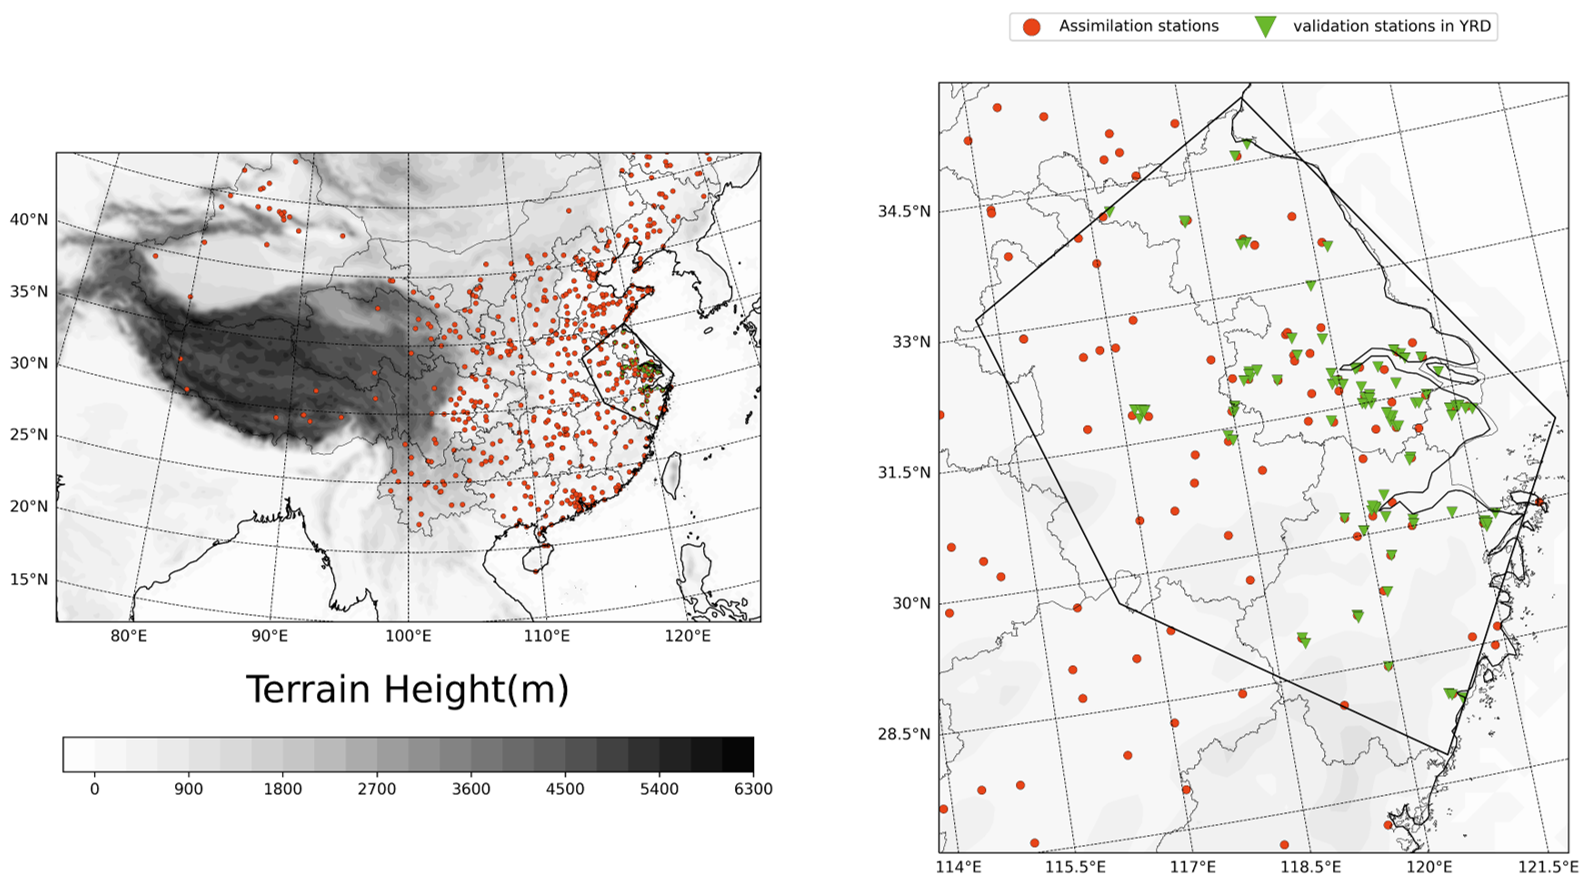
\includegraphics[width=0.8\colwidth,angle=0]{figure/domain_station_split.png}}
                    \caption{domain setting and station distribution. The left subplot shows model domain in WRF-Chem, shading shows the terrain height. Red rots represent assimilation stations, and green triangles are validation stations in Yangtze River Delta(YRD) region selected by the black polygon. The right subplot shows more detailed station distribution in YRD region.  }\label{fig1}
                \end{figure}

			\end{block}
			
			\begin{block}{Methodology for emission inversion}
				
                In order to get emission inversion, we extend emission scaling factors $\lambda$ as part of WRF-Chem model state variables, and it will be integrated by using the ensemble forecast chemical concentration fields produced by WRF-Chem. The flow chat below describes this framework.  
 
                \begin{figure}
                    \centerline{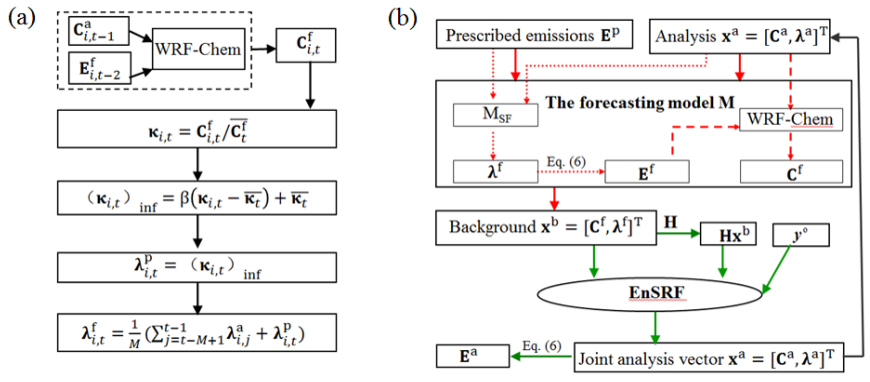
\includegraphics[width=30pc,angle=0,scale=2.5]{figure/Methodology.png}}
                    \caption{(a) describe the framework to integrate scaling factor $\lambda$. (b) flow chart of the data assimilation system that simultaneously optimizes the chemical initial
                    conditions and emissions.}\label{fig2}
                \end{figure}

                % After been integrated and assimilated, the estimated emission $E^a$ can now be calculated by prescribed emission $E^p$ and $\lambda^a$ as:
                % \begin{equation}
                %     E^a=\lambda^a*E^{p} 
                % \end{equation}
				
			
				
			\end{block}
			
			\begin{block}{VOC selection}

				
				% \begin{itemize}
				% 	\item \textbf{correlation}: 
				% 	\item \textbf{potential influence}: 
				% 	\item \textbf{Vestibulum et massa diam}. 
				% \end{itemize}
    
				\begin{figure}
                    {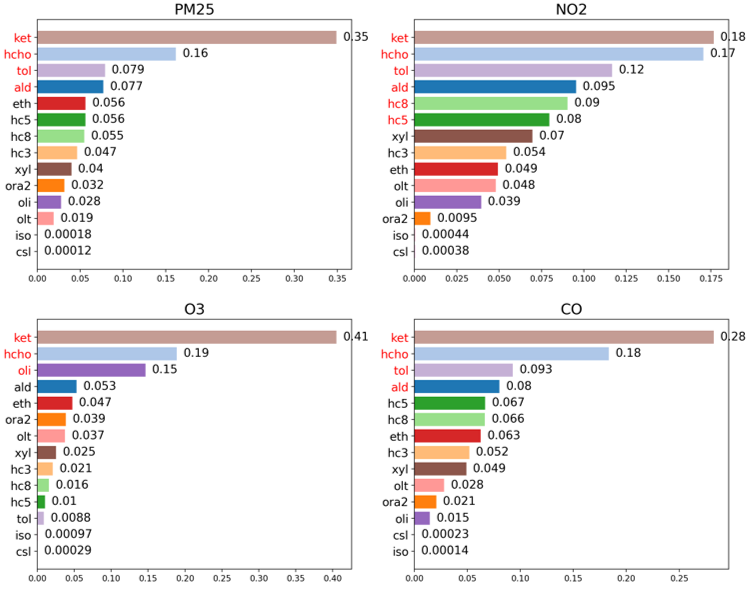
\includegraphics[width=0.6\colwidth,angle=0,scale=1]{figure/VOC_factor_domainavg.png}}
                    \caption{Normalized VOC factor for each observation kind. VOCs with a red name will be included in our assimilation system.}\label{fig_voc_factor}
                \end{figure}
                A quantified standard will make it clear to decide which VOC species should be assimilated. Here, we propose a VOC factor to quantify which VOC species should be included in the assimilation system. The VOC factor considers two parts:
                \begin{itemize}
                    \item correlation between observation and VOC species
                    \item the potential influence of updating VOC species on other variables
                \end{itemize}        
                A 50-member ensemble of free forecasts without any assimilation is conducted from 2022-07-10:00 to 2022-08-10:00 to calculate these factors(and also provide spin-up IC for cycling assimilation). Details about the calculation can be seen at the QR code in Appendix.
			\end{block}
			\begin{block}{}
			    \begin{figure}
                   \begin{minipage}[t]{0.2\colwidth}
                       
\includegraphics[scale=0.2]{logos/aerss_logo.png}
                   \end{minipage}
                   \begin{minipage}[t]{0.2\colwidth}
                       
\includegraphics[scale=0.2]{logos/aerss_logo.png}
                   \end{minipage}
                \end{figure}

			\end{block}
		\end{column}
	
		\separatorcolumn
		
		\begin{column}{\colwidth}
			
			\begin{block}{Experiment design}
               We designed four experiments to explore the effects of VOCs selection in assimilation: \texttt{no\_voc, o3\_allvoc, o3\_5pctvoc, allobs\_avgvoc}. The meteorology variables and six main pollutions(including NOx), together with the emission scaling factors, will be updated by their corresponding observations in all experiments, which is the same in \parencite{Peng_2020}. The only difference between the four experiments is the strategy to assimilate VOC species, which is shown in the table below.
                \begin{table}[t]
                    \begin{center}
                    \begin{tabular}{ccccrrcrc}
                    \hline\hline
                     & no\_voc & o3\_allvoc & o3\_5pctvoc & allobs\_avgvoc \\
                    ket & x & o3 & o3 & pm25/no2/co/o3 \\ 
                    hcho & x & o3 & o3 & pm25/no2/co/o3 \\ 
                    tol & x & o3 & x & pm25/no2/co \\ 
                    oli & x & o3 & o3 & o3 \\ 
                    ald & x & o3 & o3 & pm25/no2/co \\ 
                    hc8 & x & o3 & x & no2 \\ 
                    hc5 & x & o3 & x & no2 \\ 
                    xyl & x & o3 & x & x \\ 
                    eth & x & o3 & x & x \\ 
                    hc3 & x & o3 & x & x \\ 
                    olt & x & o3 & x & x \\ 
                    ora2 & x & o3 & x & x \\ 
                    iso & x & o3 & x & x \\ 
                    csl & x & o3 & x & x \\ 
                    \hline
                    
                    
                    \hline
                    \end{tabular}
                    
                    \end{center}
                    \caption{VOC selection table. The columns are experiments, the rows are 14 RACM VOC species. If the value is "x", this VOC will not be updated by any observation in the column experiment. If the value is observation type(s), this VOC will be updated by the given observation type(s) in the column experiment. }\label{tab_voc}
                    
                \end{table}
                Starting on Jul 22nd, every UTC00, 06, 12, 18, a deterministic 72h forecast will be launched based on the ensemble mean of cycling analysis and the posterior emission to evaluate the assimilation system.
			\end{block}
			
			\begin{alertblock}{72H ozone/PM2.5 forecast results}
				
                \begin{figure}
                    \centerline{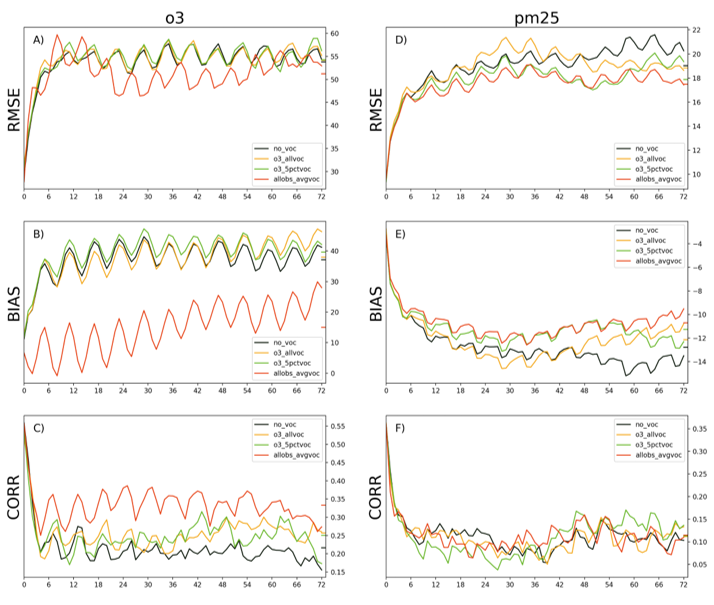
\includegraphics[width=0.8\colwidth,angle=0]{figure/fcst72h_00_6hcycle_final.png}}
                    \caption{RMSE/BIAS/CORR values averaged over all sets of forecasts. Columns are o3 and PM25, and rows are corresponding RMSE/BIAS/CORR for o3 and PM25. The right bars in each subplot represent the averaged value of RMSE/BIAS/CORR.}\label{fcst_result}
                \end{figure}
                \begin{itemize}
                    \item When using only ozone obs, a VOC selection results better RMSE and BIAS of PM2.5 forecasts.
                    
                    \item A VOC selection makes it possible to utilize 'uncorrelated' obs, and results better forecast performace for both PM2.5 and ozone.
                \end{itemize}
			\end{alertblock}
			
			\begin{alertblock}{estimated emission}
                \begin{figure}
                    \centerline{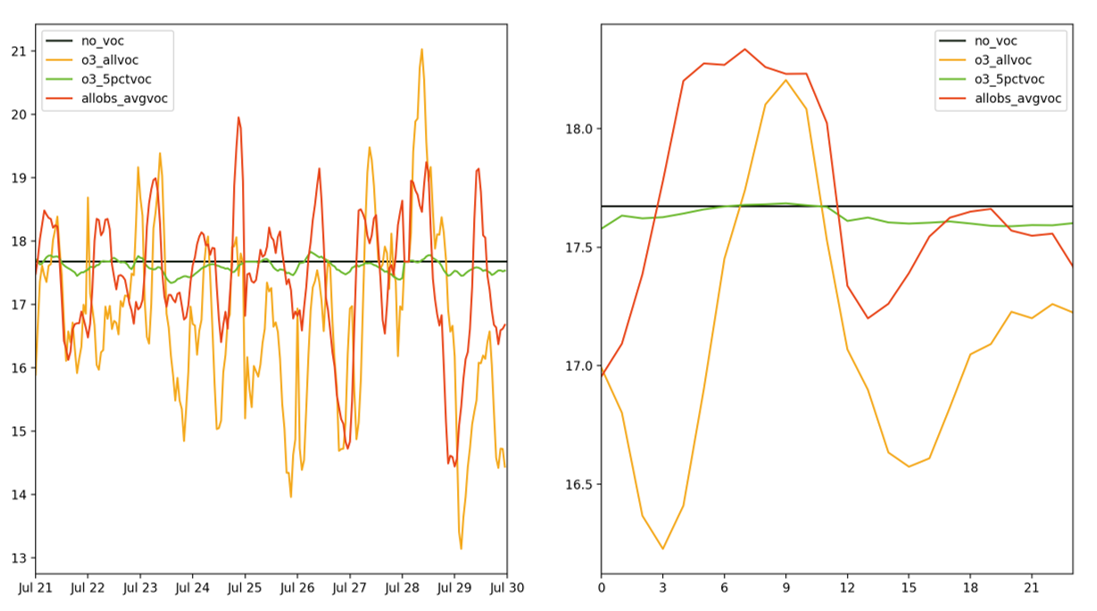
\includegraphics[width=0.8\colwidth,angle=0]{figure/POSTERIOR_emiss_timeseries_24Havg_final.png}}
                    \caption{Time series of the ensemble mean of overall VOC emissions in each experiment. The left subplot shows the whole cycling period, and the right subplot shows the time series averaged every 24H. }\label{fig_emiss_ts}
                \end{figure}
                \begin{itemize}
                    \item The "allobs\_avgvoc" emission shows an obvious daily change, with a peak during the daytime and a valley after sunset.
                    \item The daily change of VOC emission after selected updates is consistent with Ozone's daily change, and the updated emission peak in daytime can help the model to overcome the underestimation of Ozone simulation shown in \cref{fcst_result}
                \end{itemize}

			\end{alertblock}
			
		\end{column}
		
		\separatorcolumn
	\end{columns}
\end{frame}
\end{document}